\title{Лекция 8\\Представление структур и семантических окрестностей в базе знаний}   
\author[]{Шункевич Д.В.}
\institute[]{Белорусский государственный университет информатики и радиоэлектроники}

\begin{frame}
	\titlepage
\end{frame}

\begin{frame}{\\Содержание лекции}
	\topline
	\justifying
	Понятие структуры как фрагмента базы знаний. Типология структур, роли элементов структуры. Отношения на структурах. Представление в базе знаний метаинформационных конструкций. Понятие семантической окрестности, типология семантических окрестностей.
\end{frame}

\begin{frame}{Понятие структуры как фрагмента базы знаний}
	\topline
	\justifying
	При накоплении больших	объемов информации в базе знаний возникает необходимость выделять \textbf{целые фрагменты} базы знаний и иметь возможность их специфицировать, рассматривая \textbf{как отдельные сущности}.
	
	Такой фрагмент базы знаний назван структурой (sc-структурой).
	
	Под \textbf{\textit{структурой}} будем понимать \textbf{множество
	sc-элементов}, удаление одного из которых может привести к нарушению целостности этого множества.

	Структура может изображаться путем явного указания всех пар принадлежности элементов этой структуре, а также в виде контура, содержащего все элементы, входящие в состав этой структуры.
\end{frame}

\begin{frame}{Пример представления структуры как фрагмента базы знаний}
	\topline
	\justifying
	\begin{figure}[H]
		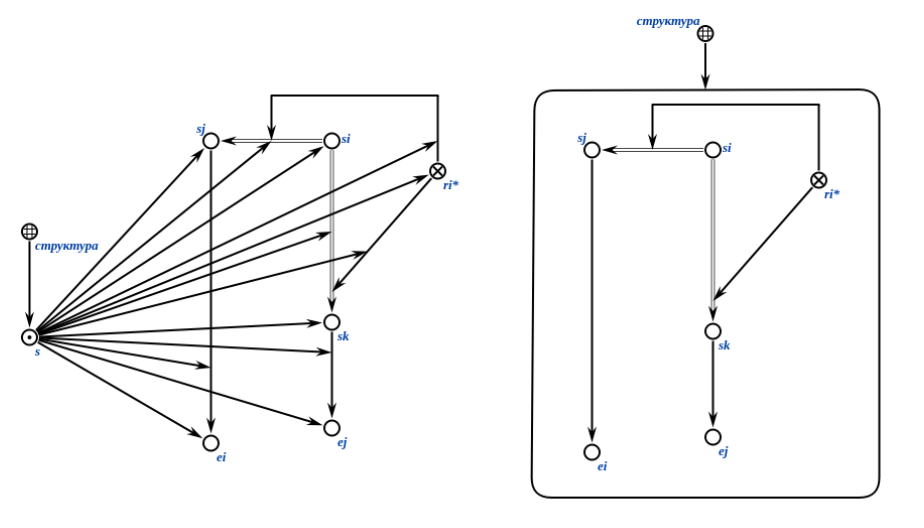
\includegraphics[scale=0.33]{./figures/sd_structures/structure.png}
	\end{figure}
\end{frame}

\begin{frame}{\\Типология структур}
	\topline
	\justifying
	\begin{SCn}
	\scnheader{структура}
	\begin{scnrelfromset}{разбиение}
		\scnitem{связная структура}
		\scnitem{несвязная структура}
	\end{scnrelfromset}
	\begin{scnrelfromset}{разбиение}
		\scnitem{тривиальная структура}
		\begin{scnindent}
			\scnidtf{структура, не содержащая связок}
		\end{scnindent}
		\scnitem{нетривиальная структура}
		\begin{scnindent}
			\scnidtf{структура, содержащая хотя бы одну связку}
		\end{scnindent}
	\end{scnrelfromset}
	\end{SCn}
\end{frame}


\begin{frame}{\\Типология структур}
	\topline
	\justifying
	Структуре, представленной в SC-коде, поставим в соответствие орграф, вершинами которого являются sc-элементы, а дугами -- связки отношений инцидентности, связывающие sc-коннекторы с инцидентными им sc-элементами, которые являются компонентами указанных sc-коннекторов. Если полученный таким способом орграф является связным орграфом, то исходную структуру будем считать связной структурой.
	
	Если полученный	таким способом орграф не является связным орграфом, то исходную структуру будем считать несвязной структурой.
\end{frame}


\begin{frame}{\\Типология структур}
	\topline
	\justifying
	\vspace{10mm}
	
	По признаку стационарности выделяются динамические структуры (процессы),	состав которых меняется с течением времени, и статические структуры, состав которых не меняется	с течением времени.
	
	\begin{SCn}
	\scnheader{структура}
	\begin{scnrelfromset}{разбиение}
		\scnitem{процесс}
		\begin{scnindent}
			\scnidtf{динамическая структура}
			\scnidtf{нестационарная структура}
		\end{scnindent}
		\scnitem{статическая структура}
		\begin{scnindent}
			\scnidtf{стационарная структура}
			\scnidtf{структура, не изменяющаяся во времени}
		\end{scnindent}
	\end{scnrelfromset}
	\end{SCn}
\end{frame}

\begin{frame}{\\Типология структур}
	\topline
	\justifying
	
	По признаку времени существования выделяются временные структуры и постоянно существующие структуры.

	\begin{SCn}
	\scnheader{структура}
	\begin{scnrelfromset}{разбиение}
		\scnitem{временная структура}
		\scnitem{постоянно существующая структура}
	\end{scnrelfromset}
	\end{SCn}
\end{frame}

\begin{frame}{\\Роли элементов структуры}
	\topline
	\justifying
	\vspace{10mm}
	
	Для формального представления структур используются понятия, описывающие роли элементов в рамках структуры. \textbf{\textit{элемент структуры\scnrolesign}} -- неосновное понятие, ролевое отношение, указывающее на все элементы каждой структуры.
	
	\begin{SCn}
	\scnheader{элемент структуры\scnrolesign}
	\begin{scnrelfromset}{разбиение}
		\scnitem{непредставленное множество\scnrolesign}
		\scnitem{полностью представленное множество\scnrolesign}
		\scnitem{частично представленное множество\scnrolesign}
		\scnitem{элемент структуры, не являющийся множеством\scnrolesign}
	\end{scnrelfromset}
	\end{SCn}
\end{frame}

\begin{frame}{\\Роли элементов структуры}
	\topline
	\justifying
	\vspace{10mm}
	
	\begin{SCn}
	\scnheader{элемент структуры\scnrolesign}
	\begin{scnrelfromset}{разбиение}
		\scnitem{максимальное множество\scnrolesign}
		\begin{scnindent}
			\scntext{пояснение}{Ролевое отношение, связывающее структуру со знаком множества, для которого не существует множества, которое было бы надмножеством указанного множества и знак которого был бы элементом этой же структуры}
		\end{scnindent}
		\scnitem{немаксимальное множество\scnrolesign}
		\begin{scnindent}
			\scntext{пояснение}{Ролевое отношение, связывающее структуру со знаком множества, для которого в рамках данной структуры существует множество, являющееся надмножеством указанного множества.}
		\end{scnindent}
	\end{scnrelfromset}
	\end{SCn}
\end{frame}

\begin{frame}{\\Роли элементов структуры}
	\topline
	\justifying
	\vspace{5mm}
	
	\begin{SCn}
	\small
	\scnheader{элемент структуры\scnrolesign}
	\begin{scnrelfromset}{разбиение}
		\scnitem{первичный элемент\scnrolesign}
		\begin{scnindent}
			\scntext{пояснение}{Ролевое отношение, указывающее на (атомарный) элемент структуры, который не имеет элементов, ему принадлежащих. При этом	соответствующая пара принадлежности может существовать, но в состав данной структуры не входить.}
		\end{scnindent}
		\scnitem{вторичный элемент\scnrolesign}
		\begin{scnindent}
			\scnidtf{элемент данной структуры имеющий семантический уровень более 2\scnrolesign}
			\scnidtf{непервичный элемент\scnrolesign}
			\scntext{пояснение}{Ролевое отношение, указывающее на элемент структуры, обозначающий множество элементов, где обязательно хотя бы один элемент указанного множества входил бы в указанную структуру.}
		\end{scnindent}
	\end{scnrelfromset}
	\end{SCn}
\end{frame}

\begin{frame}{\\Роли элементов структуры}
	\topline
	\justifying
	
	\scnheader{элемент структуры\scnrolesign}
	\begin{scnrelfromset}{разбиение}
		\scnitem{структура первого уровня\scnrolesign}
		\begin{scnindent}
			\scntext{пояснение}{связка первичных элементов, тривиальная структура из первичных элементов или класс первичных элементов}
		\end{scnindent}
		\scnitem{вторичная структура\scnrolesign}
		\begin{scnindent}
			\scntext{пояснение}{структура, среди элементов которой есть хотя бы один вторичный элемент\scnrolesign}
		\end{scnindent}
	\end{scnrelfromset}
\end{frame}

\begin{frame}{\\Пример ролей элементов структуры}
	\topline
	\justifying
	\begin{figure}[H]
		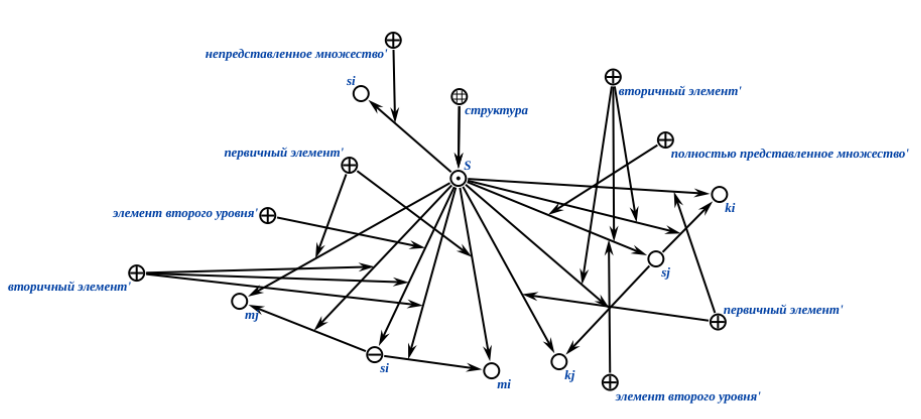
\includegraphics[scale=0.37]{./figures/sd_structures/roles.png}
	\end{figure}
\end{frame}

\begin{frame}{\\Отношения на структурах}
	\topline
	\justifying
	\scnheader{бинарное отношение*}
	\scnhaselement{полиморфность* }
		\begin{scnindent}
			\scnsubset{соответствие*}
		\end{scnindent}
	\scnhaselement{полиморфизм*}
	\scnhaselement{гомоморфность*}
		\begin{scnindent}
		\scnsubset{соответствие*}
		\end{scnindent}
	\scnhaselement{гомоморфизм*}
	\scnhaselement{изоморфность*}
		\begin{scnindent}
		\scnsubset{соответствие*}
		\end{scnindent}
	\scnhaselement{изоморфизм*}
	\scnhaselement{автомоморфность*}
		\begin{scnindent}
		\scnsubset{соответствие*}
		\end{scnindent}
	\scnhaselement{автоморфизм*}
\end{frame}

\begin{frame}{\\Отношения на структурах}
	\topline
	\justifying
	
	\scnheader{полиморфность* }
	\scntext{пояснение}{полиморфность* -- это соответствие, заданное на структурах, при котором каждому элементу из области	определения соответствия (первой структуры) ставится в соответствие один или более элемент из области значения соответствия (второй структуры), при этом существует хотя бы один элемент области определения	соответствия, которому соответствуют два или более элемента из области значения соответствия.}
\end{frame}

\begin{frame}{\\Отношения на структурах}
	\topline
	\justifying
	
	\scnheader{гомоморфность*}
	\scntext{пояснение}{гомоморфность* -- это соответствие, заданное на структурах, при котором каждому элементу из области	определения соответствия (первой структуры) ставится в соответствие только один элемент из области		значения соответствия (второй структуры).}
\end{frame}

\begin{frame}{\\Отношения на структурах}
	\topline
	\justifying
	
	\scnheader{изоморфность*}
	\scntext{пояснение}{изоморфность* -- это гомоморфность*, при которой для каждого элемента из области значения существует	ровно один соответствующий элемент из области определения.}
	
	
	\scnheader{автомоморфность*}
	\scntext{пояснение}{автоморфность* -- это изоморфность*, у которой область определения соответствия и область значения соответствия совпадают.}
\end{frame}

\begin{frame}{\\Отношения на структурах}
	\topline
	\justifying
	
	\scnheader{аналогичность структур*}
	\scnsubset{соответствие*}
	\scniselement{бинарное отношение*}
	\scntext{пояснение}{аналогичность структур* -- соответствие*, задаваемое на структурах, и фиксирующее факт наличия некоторой
	аналогии на подструктурах (подмножествах) указанных структур. Каждой ориентированной паре, принадлежащей аналогичности структур* может быть поставлено в соответствие множество пар, задающих сходства*	некоторых подструктур и различия* некоторых подструктур исходных структур.}
\end{frame}

\begin{frame}{\\Пример}
	\topline
	\justifying
	
	\begin{figure}[b]
		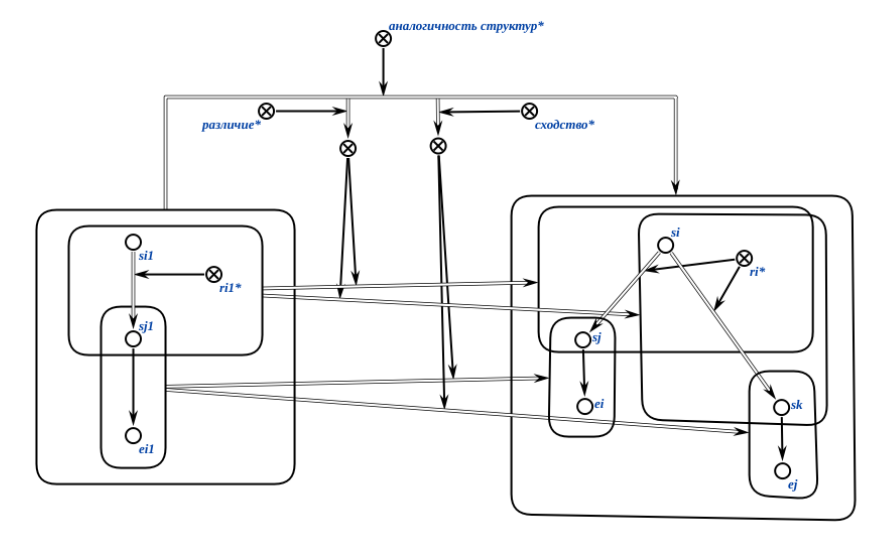
\includegraphics[scale=0.3]{./figures/sd_structures/analog.png}
	\end{figure}
\end{frame}

\begin{frame}{\\Понятие семантической окрестности}
	\topline
	\justifying
	
	\vspace{5mm}
	Для спецификации отдельных сущностей в рамках базы знаний вводится понятие \textit{\textbf{семантической окрестности}}.
	
	Семантическая окрестность представляет собой спецификацию заданной сущности, знак которой указывается	как ключевой элемент этой спецификации. В отличие от других видов знаний, семантическая окрестность имеет только один ключевой элемент.
	
	Набор признаков, по которым можно специфицировать сущности, различен. Кроме того, может возникнуть необходимость специфицировать одну и ту же сущность в различных аспектах и явно фиксировать эти аспекты в базе знаний.
	
	Так, например, одну и ту же персону можно описывать с профессиональной, медицинской, гражданской и других точек зрения.
\end{frame}

\begin{frame}{\\Пример}
	\topline
	\justifying
	\vspace{10mm}
	
	\begin{figure}[H]
		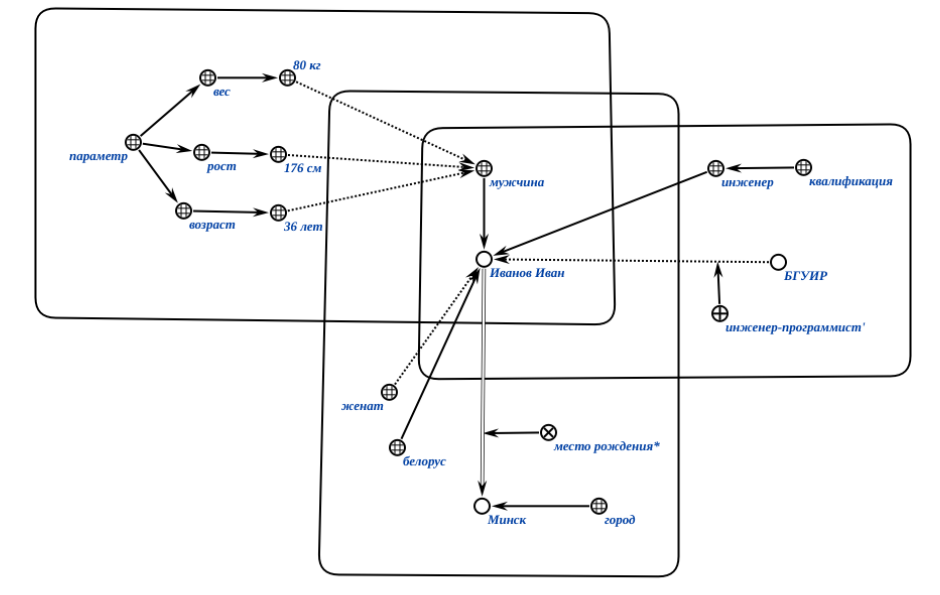
\includegraphics[scale=0.35]{./figures/sd_structures/example.png}
	\end{figure}
\end{frame}

\begin{frame}{\\Понятие семантической окрестности}
	\topline
	\justifying
	
	\begin{SCn}
	\scnheader{семантическая окрестность}
	\scnidtf{описание заданной сущности, знак которой указывается как ключевой элемент этой спецификации}
	\scnsubset{знание}
	\scnsuperset{семантическая окрестность по инцидентным коннекторам}
	\scnsuperset{полная семантическая окрестность}
	\scnsuperset{базовая семантическая окрестность}
	\scnsuperset{специализированная семантическая окрестность}
	\end{SCn}

\end{frame}

\begin{frame}{\\Типология семантических окрестностей}
	\topline
	\justifying
	
	\begin{SCn}
	\scnheader{семантическая окрестность по инцидентным коннекторам}
	\scnsuperset{семантическая окрестность по выходящим дугам}
	\scnsuperset{семантическая окрестность по входящим дугам}
	\scntext{пояснение}{вид семантической окрестности, в которую входят все коннекторы, инцидентные заданному элементу, а также
	все элементы, инцидентные указанным коннекторам.}
	\end{SCn}

\end{frame}

\begin{frame}{\\Типология семантических окрестностей}
	\topline
	\justifying
	
	\begin{SCn}
	\scnheader{полная семантическая окрестность}
	\scnidtf{полная спецификация некоторой описываемой сущности}
	
	\scnheader{базовая семантическая окрестность}
	\scnidtf{минимально достаточная семантическая окрестность}
	
	\scnheader{специализированная семантическая окрестность}
	\scnidtf{вид семантической окрестности, набор связей для которой уточняется отдельно для каждого типа такой окрестности.}
	\end{SCn}

\end{frame}

\begin{frame}{\\Типология семантических окрестностей}
	\topline
	\justifying
	
	\begin{SCn}
	\scnheader{специализированная семантическая окрестность}
	\scnsuperset{пояснение}
	\scnsuperset{примечание}
	\scnsuperset{правило идентификации экземпляров}
	\scnsuperset{терминологическая семантическая окрестность}
	\scnsuperset{теоретико-множественная семантическая окрестность}
	\scnsuperset{логическая семантическая окрестность}
	\scnsuperset{описание типичного экземпляра}
	\scnsuperset{описание декомпозиции}
	\end{SCn}
	
\end{frame}

